
Todas as informações dadas a seguir se referem ao que foi adotado no projeto submetido e aceito. Legendas de figuras ficam abaixo da figura (veja a Figura \ref{fig:aminosequence}). Legendas de tabelas ficam acima (veja Tabela \ref{tab:cronograma}).

Figuras podem ser justapostas, e cada figura recebe sua própria legenda, como visto nas Figuras \ref{fig:aminosequence} e \ref{fig:peptidebond}. No entanto, posicioná-las corretamente não é simples, então cuidado deve ser tomado. Em especial, atenção com os caracteres "\%" posicionados no final de certas linhas no arquivo latex deste projeto, pois eles são importantes para o correto funcionamento do ambiente \textit{minipage}.

\begin{figure}[htb]
\centering
\begin{minipage}{.4\textwidth}
  \centering
  \vspace{1cm}
  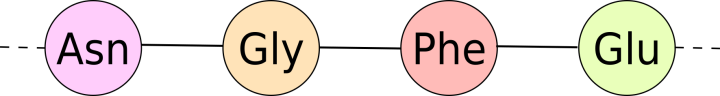
\includegraphics[width=0.8\textwidth]{imagens/amino_seq.png}
  \vspace{1cm}
  \captionof{figure}{Uma sequência dos aminoácidos: asparagina, glicina, fenilalanina e ácido glutâmico.}
  \label{fig:aminosequence}
\end{minipage}%
\hspace{.04\textwidth}%
\begin{minipage}{.55\textwidth}
  \centering
  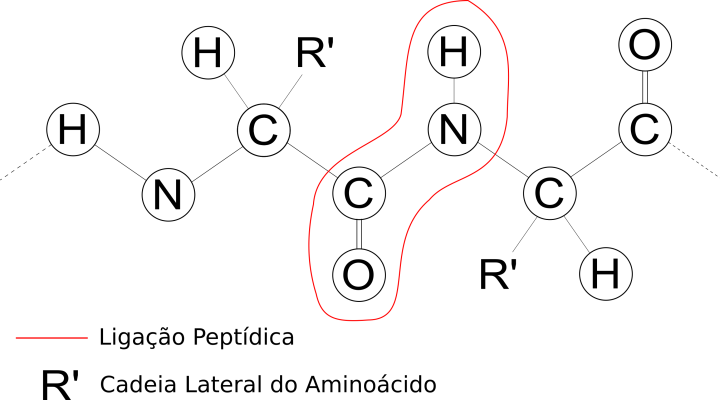
\includegraphics[width=0.8\linewidth]{imagens/protein_planar_pepbond.png}
  \captionof{figure}{Dois aminoácidos ligados por uma ligação peptídica.}
  \label{fig:peptidebond}
\end{minipage}
\end{figure}

Figuras retiradas de fontes externas devem ter sua fonte citada na legenda da mesma; caso contrário, poderia configurar plágio. Na Figura \ref{fig:hemoglobin3d}, a fonte é citada e uma URL é fornecida via nota de rodapé.

\begin{figure}[htb]
    \centering
    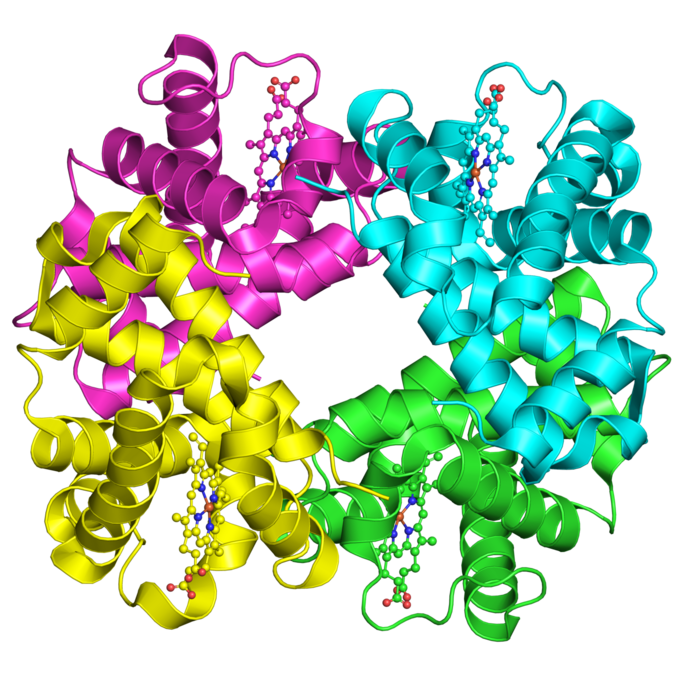
\includegraphics[width=0.35\linewidth]{imagens/3d_hemoglobin.png}
    \caption{Estrutura tridimensional da hemoglobina, obtida de \textit{Protein Data Bank in Europe} \protect\footnotemark{}.}
    \label{fig:hemoglobin3d}
\end{figure}

% Completa o \footnotemark utilizado na legenda da figura acima.
\footnotetext{https://www.ebi.ac.uk/pdbe/entry/pdb/1a3n}

Quando precisar de um pedaço qualquer de texto para preencher qualquer lugar temporariamente, pode-se usar o comando \textit{lipsum}, que resulta no parágrafo a seguir.

\lipsum[1]

Caso tenha algum parágrafo que precisa ser revisado futuramente, pode-se usar o comando \textit{rev}. Por exemplo, \rev{este texto precisa ser revisado}.